\glsreset{clf}\glsreset{cbf}
Based on \citep{bib:artstein}, who founded \gls{clf}s, a \gls{cbf} can be created \citep{bib:org_control}. With a system $\dot{x}=f(x)+g(x)u$, a \gls{cbf} exist if the below constraints are fulfilled:
\begin{exa}
\begin{flalign}
& x\in \mathcal{X}_u \hspace{0.3cm} \Rightarrow \hspace{0.3cm} B(x) > 0  \label{req1} \\
& L_gB(x) = 0 \hspace{0.3cm} \Rightarrow \hspace{0.3cm} L_fB(x) < 0 \label{req2} \\
& \{ x \in \mathcal{X} | B(x) \leq 0 \} \neq \emptyset \label{req3}
\end{flalign}
\vspace{-0.6cm}
\begin{longtable}{p{.9\textwidth} p{.1\textwidth} p{.1\textwidth}} 
Where  & & \\
$B(x)$ is a control barrier function & [$\cdot$] \\ 
$L_fB(x)$ is the Lie derivative of $B(x)$ along the vector field  $f(x)$, i.e. $\frac{\partial B(x)}{\partial x}f(x)$ & [$\cdot$] \\ 
$L_gB(x)$ is the Lie derivative of $B(x)$ along the vector field  $g(x)$, i.e. $\frac{\partial B(x)}{\partial x}g(x)$ & [$\cdot$] 
\end{longtable}
\vspace*{-0.2cm}
\end{exa}
Taking a look at \autoref{req1} it states essentially the same as \autoref{cer2}, i.e. the unsafe area exist whenever $B(x)>0$. This makes it possible to design an unsafe region. \Autoref{req2} put forth the requirement that the gradient along the vector field $f(x)$ must point away from the barrier extremities whenever the input is with no significance (except for the critical point). \Autoref{req3} simply states that the safe area must contain some states as control otherwise is impossible.

This chapter intends to implement and analyse a controller ensuring safety if the demands from \autoref{req1}, \ref{req2} and \ref{req3} are obeyed. This shall first be tested on the slide movement on the Da Vinci surgical robot as it composes a prismatic joint and a 1:1 mapping from slide $joint\_angle$ to 1D position. Hence any inverse kinematic solver can be bypassed in the early phase of this project which is an important simplification to eliminate initial complications.
\subsection{Overview}
The slide movement is visualized in \autoref{fig:slidefig} and an overview of terms used in this section is found in \autoref{fig:safe:overview}. \Autoref{fig:safe:overview} encompasses likewise the case study considered in this chapter. It put forth the demands that the upper region, i.e. the interval $[\Lambda_{h+}:\Lambda_\text{lim+}]$ is an unsafe area and the rest is considered safe. Furthermore, everything outside the slide physical limits, i.e. $[-\infty:\Lambda_\text{lim-}]$ and $[\Lambda_\text{lim+}:\infty]$ is also considered unsafe. This case study is purely made up with the purpose to demonstrate the use of a safety controller.
\begin{figure}[H]
    \centering
    \begin{minipage}{.5\textwidth}
        \centering
        \includegraphics[width=0.73\linewidth]{slidemovefigure.pdf}
        \caption{Illustration of slide movement.}
        \label{fig:slidefig}
    \end{minipage}%
    \begin{minipage}{0.5\textwidth}
        \centering
        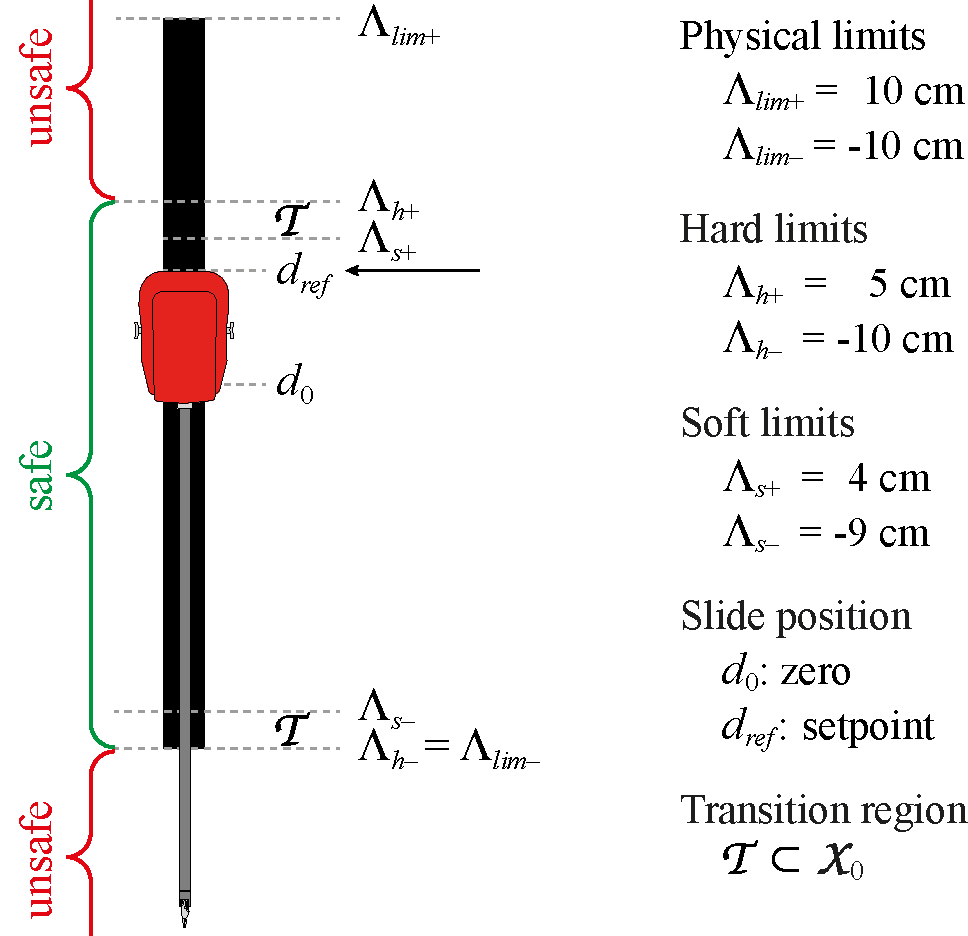
\includegraphics[width=0.7\linewidth]{slide_overview.pdf}
        \caption{Boundaries used in this section.}
        \label{fig:safe:overview}
    \end{minipage}
\end{figure}
At this point, a system model is required before any controller design may be initiated.
%\hspace{1cm }\texttt{rostopic echo joint\_states/position[6]} \hspace{0.2cm} {\color{blue}{\# Be sure to have the ROS environment correctly configured according to \autoref{app:ros}}}
\section{Modelling of Slide Movement}
To obtain a model of the slide movement, the step response will be measured.  This can be done by subscribing to the \texttt{joint\_state} topic in \gls{ros}. The experiment is described in further details in \autoref{app:meas}. The result is plotted in \autoref{fig:stepresponseslide}. 
\begin{figure}[H]
\center
\includegraphics[scale=0.5]{step_slide.eps}
\caption{Step response from 0\,mm to 5\,mm. Plot details and measurements can be found in \autoref{app:cd} as \texttt{matlab\_scripts/slide\_step/plot\_slide\_pos.m}. The experiment is described in \autoref{app:meas}.}
\label{fig:stepresponseslide}
\end{figure}
The system can clearly be well approximated with an underdamped second order model, however, for initial simplicity, merely a simple model of the slide movement is used. It shall, however, also be approximated with as a second order system. This introduces a number of other challenges which is the reason for initial simplicity. These models will throughout this chapter be referenced as:
\begin{itemize}
\item One dimensional (1D) model
\item Two dimensional (2D) model
\end{itemize}
\subsection{One Dimensional Model based on Position}
The system can be approximated to a linear first order system with a dominating time constant \gls{taus}. The time constant is read from \autoref{fig:stepresponseslide}:
\begin{flalign*}
\tau_s = 110\, \text{ms}
\end{flalign*} 
A linear system can be outlined as:
\begin{flalign*}
& Y(s) = \dfrac{1}{\tau_s s + 1}U(s) =  \dfrac{1/\tau_s}{s + 1/\tau_s}\,U(s) = (s+1/\tau_s)^{-1}\,1/\tau_s\,U(s) \kk  \overset{\overset{Y(s)=(C(sI-A)^{-1}B+D)U(s)}{\longrightarrow}}{\scriptsize \text{compare to obtain SS form}}  \\ 
& \dot{x} = \underbrace{-\tau_s^{-1}\,x}_{Ax} + \underbrace{\tau_s^{-1}}_{B} u
\end{flalign*}
The system matrix $A$ and the input matrix $B$ can be read from the above equation:
\begin{flalign*}
A = - \tau_s^{-1} =  \kk \wedge \kk B = \tau_s^{-1} \kk \wedge \kk C = 1 \kk \wedge \kk D = 0
\end{flalign*}
Which completes the first order approximation.
\subsection{Two Dimensional Model based on Position and Velocity}
The second order approximation is based on the form:
\begin{flalign}
\dfrac{Y(s)}{U(s)} = \dfrac{\omega_n^2}{s^2 + 2\zeta \omega_n s + \omega_n^2}
\label{eq:2order}
\end{flalign}\\
\vspace{-0.6cm}
\begin{longtable}{p{.9\textwidth} p{.1\textwidth} p{.1\textwidth}} 
Where  & & \\
$Y(s)$ is the output in the Laplace domain  & [m] \\
$U(s)$ is the input in the Laplace domain  & [m] \\
$\omega_n$ is the natural frequency of the system & [rad/s] \\
$\zeta$ is the damping coefficient  & [$\cdot$] \\
$s$ is the Laplace operator  & [rad/s] 
\end{longtable}
\vspace*{-0.2cm}
The model can unambiguous be approximated from the rise time $t_r$, settling time $t_s$ (5\,\% settling time) and the overshoot $M_p$ \citep{bib:dynamicsystems}. They are measured with the purpose to find $\omega_n$ and $\zeta$:
\begin{flalign*}
\omega_n = \dfrac{1.8}{t_r} = \dfrac{1.8}{0.106\,\text{s}} = 17 \,\text{rad/s} \kk \wedge \kk  \zeta = \dfrac{1}{\omega_n \cdot t_s}\log (0.05) = \dfrac{1}{17 \cdot 0.320}\log(0.05) = 0.55
\end{flalign*}
\Autoref{eq:2order} can be transferred to state space form:
\begin{flalign*}
&Y(s)s^2 + 2\zeta \omega_n Y(s) s + \omega_n^2 Y(s) - \omega_n^2 U(s)  = 0 \\
&\ddot{y}(t) + 2\zeta \omega_n \dot{y}(t) + \omega_n^2 y(t) - \omega_n^2 u(t) = 0 \\
&\text{choose $y(t) = x_1(t) = \text{position} \kk \Rightarrow \kk \dot{x}_1(t) = x_2(t)$} \\
&\begin{bmatrix}
\dot{x}_2(t)\\\dot{x}_1(t)
\end{bmatrix} = \begin{bmatrix}
-2\zeta \omega_n & -\omega_n^2 \\
1 & 0 
\end{bmatrix}\begin{bmatrix}
x_2(t) \\ x_1(t)
\end{bmatrix} + \begin{bmatrix}
1\\0
\end{bmatrix}u(t) \\
&\hspace{0.65cm}y(t) = \begin{bmatrix}
0 & \omega_n^2
\end{bmatrix}\begin{bmatrix}
x_2(t) \\ x_1(t)
\end{bmatrix}
\end{flalign*}
\vspace{-0.6cm}
\begin{longtable}{p{.8\textwidth} p{.1\textwidth} p{.1\textwidth}} 
Where  & & \\
$x_1(t)$ is the position (attenuated by $\omega_n^2$) & [m] \\
$x_2(t) = \dot{x}_1(t)$ is the velocity  & [m/s] \\
$y(t)$ is the output (slide position)  & [m] \\
$u(t)$ is the control input  & [$\cdot$]
\end{longtable}
\vspace*{-0.2cm}
Thus:
\begin{flalign*}
A = \begin{bmatrix}
-2\zeta \omega_n & -\omega_n^2 \\
1 & 0 
\end{bmatrix} \kk \wedge \kk B = \begin{bmatrix}
1 \\ 0
\end{bmatrix} \kk \wedge \kk C = \begin{bmatrix}
0 & \omega_n^2
\end{bmatrix} \kk \wedge \kk D = 0
\end{flalign*}
Which completes the second order model.
\section{Construction of CBF}
To illustrate the usefulness of \gls{cbf}s, a palpable example hereof will be created with direct application to the Da Vinci robot. This example does not directly constitute application to a patient but favour the theory in a neat and comprehensible sense and secure a way to visually and physically verify the method.

Consider the state intervals defined in \autoref{tab:intervals}.
\begin{table}[H]
	\begin{tabularx}{\textwidth}{X X X }
\rowcolor{HeaderBlue} 
$\mathcal{X}$ & $\mathcal{X}_u$  & $\mathcal{X}_0$ \\
$x \in \{[\Lambda_{s+}:\Lambda_\text{lim+}],[\Lambda_\text{lim-}:\Lambda_{s-}]\}$  & $x \in \{[\Lambda_{h+}:\Lambda_\text{lim+}],[\Lambda_\text{lim-}:\Lambda_{h-}]\} $ & $x \in \{[\Lambda_{s+}:\Lambda_{lim+}],[\Lambda_\text{lim-}:\Lambda_{s-}]\}$  \\
\end{tabularx}
\caption{Global state intervals where: $\Lambda_\text{lim}$ is the physical slide limit ($\pm$0.1\,m), $\Lambda_s$ is a soft limit denoting a transition area and $\Lambda_h$ is a hard limit where a trajectory at all cost can not cross. The interval $x \in [\Lambda_{s-}:\Lambda_{s+}]$ is safe thus any control law can be used in that area.}
\label{tab:intervals}
\end{table}
\subsection{Construction of CBF based on 1D model}
A parabola is now introduced as \gls{cbf}. A coordinate shift is performed such that the slide movement occurs along the $x$-axis instead of the $z$-axis. 
\begin{flalign*}
B(x) = ax^2+bx+c \kk \Rightarrow \kk L_fB(x) = \dfrac{d}{dx}B(x)f(x) = (2ax+b)(-\tau^{-1}x) = -2\tau^{-1}ax^2-\tau^{-1}bx
\end{flalign*}
\Autoref{req2} put forth the demand that $L_fB(x)<0$ when $L_gB(x) = 0$ as the input in that case will be insignificant. Ensuring that $L_fB(x)<0$ in the area $x \in [\Lambda_s:\Lambda_h]$ is therefore indeed sufficient. Analysis of $L_fB(x)$ shall reveal when $L_fB(x)>0$, i.e. to ensure the demand below:
\begin{flalign*}
L_fB(x) \ngeq 0\hspace{0.3cm}\forall\hspace{0.3cm} x \in [\Lambda_s:\Lambda_h]
\end{flalign*}
Thus the analysis is performed:
\begin{flalign}
L_fB(x) < 0 \kk \Leftrightarrow \kk -2\tau^{-1}ax^2-\tau^{-1}bx < 0
\label{eq:analysis}
\end{flalign}
The coefficients $a$ and $b$ must be found. By studying $x>0$ it can from \autoref{eq:analysis} be seen that:
\begin{flalign*}
\forall \mm \{ a > 0 \mm  \wedge \mm b > 0 \} \mm \Rightarrow \mm L_fB(x) < 0 \mm \forall \mm  x > 0
\end{flalign*}
The scenario changes when $x<0$. Preserving that $a>0$ and $b>0$, the analysis below put forth constraints to $x$.
\begin{flalign}
&L_fB(x) = 0 \kk \Leftrightarrow \kk  -2\tau^{-1}ax^2-\tau^{-1}bx = 0 \nonumber
 \\  &-2ax^2-bx = 0 \mm \Rightarrow \mm x = 
\begin{cases}
  \frac{-b}{2a} \\
   0,             
\end{cases}
\label{eq:interval1}
\end{flalign}
Thus, if $L_gB(x) = 0$, then $B(x)$ is not a valid barrier function within the interval:
\begin{flalign}
B(x) \hspace{0.15cm} \text{invalid:} \mm  x \in \left[ \frac{-b}{2a}:0 \right] \mm \text{if} \mm L_gB(x) = 0
\label{eq:interval}
\end{flalign}
Three equations with three unknowns can be outlined to fulfil the initial demand in \autoref{fig:safe:overview}.
\begin{flalign*}
 \left.
 \begin{aligned}
a\,\Lambda_h^2 + b\,\Lambda_h + c = 0 \\
a\,(-\Lambda_\text{lim})^2 + b\,(-\Lambda_\text{lim})^2 + c = 0 \\
a\left( \frac{-\Lambda_\text{lim}+\Lambda_h}{2}\right)^2 + b\left(\frac{-\Lambda_\text{lim}+\Lambda_h}{2}\right) + c = \underbrace{-0.025}_\text{any constant $<0$} 
\end{aligned}
\mm \right\}
 \qquad \begin{matrix}
 a &= \,\,\,\,\,\,\,\,1.7778 \\ b &= \,\,\,\,\,\,\,\,0.0889 \\ c &= -0.0089
 \end{matrix}
\end{flalign*}
The interval where $B(x)$ is invalid can thereby be found from \autoref{eq:interval}:
\begin{flalign*}
B(x) \hspace{0.15cm} \text{invalid:} \mm  x \in [-0.0250:0] \kk \text{if} \mm L_gB(x) = 0
\end{flalign*}
This is indifferent as $\mathcal{X}  \notin [\Lambda_{s-}:\Lambda_{s+}]$. Thus the barrier function is a valid \gls{cbf}. It is plotted in \autoref{fig:barrierfunction}
\begin{figure}[H]
\center
	\includegraphics[scale=0.5]{parabel_1.eps}
	\caption{Barrier function along with the $\mathcal{X}_u$ and $\mathcal{X}_u^c$. Plot details and MATLAB script can be found in \autoref{app:cd} as \texttt{matlab\_scripts/plot\_parabola/plot\_parabola.m}}
	\label{fig:barrierfunction}
\end{figure}
\underline{Note:} The above analysis ensures safety regardless of $L_gB(x) = 0$ at all time except when $L_gB(x)=0$ which merely takes place at the critical point, i.e.:
\begin{flalign*}
 L_gB(x) = (2ax+b)B = 2ax\tau^{-1} + b\tau^{-1} = 0 \kk \Leftrightarrow \kk 2ax = -b \kk \Leftrightarrow \kk x = \dfrac{-b}{2a}
 \end{flalign*} 
 This is again the parabola extremity as it was found in \autoref{eq:interval1} and in fact an allowed exception for condition \autoref{req2} as the system is in its equilibrium.
 \subsection{Construction of CBF based on 2D model}
\section{Controller Design}
A control law is now introduced:
\begin{flalign*}
u(x) =
\begin{cases}
	\bar{N}\,x_\text{ref} - K\,x \kk &\text{if \mm $x \in [\Lambda_{s-}:\Lambda_{s+}]$}\\
	 k_0(x)  \kk &\text{if \mm $x \in [\Lambda_{s+}:\Lambda_{h+}] \mm \wedge \mm x \in [\Lambda_{h-}:\Lambda_{s-}]$}
\end{cases}
\end{flalign*}
This can be combined by the control law below which is a linear combination of the two controllers.
\begin{flalign*}
u(x) &= \sigma(x)k_0(x)+(1-\sigma(x))\tilde{u}(x) \\
 &= \sigma(x)k_0(x)+(1-\sigma(x))(\bar{N} \cdot x_\text{ref}-Kx) 
\end{flalign*}
\vspace{-0.8cm}
\begin{longtable}{p{.9\textwidth} p{.1\textwidth} p{.1\textwidth}} 
Where  & & \\
$u(x) \in \mathbb{R}^{1 \times 1} $ is a control signal where safety is ensured  & [$\cdot$] \\
$\tilde{u}(x) \in \mathbb{R}^{1 \times 1}$ is a control signal to the linear state space system such that $\tilde{u}=\bar{N}\cdot x_\text{ref}-Kx $ & [$\cdot$] \\ 
$k_0(x) \in \mathbb{R}^{1 \times 1}$ is a control law that guarantees safety & [$\cdot$] \\ 
$\sigma(x) \in \mathbb{R}^{1 \times 1}$ is a parameter that founds a linear combination between the two control inputs & [$\cdot$] \\ 
$K \in \mathbb{R}^{1 \times 1}$ is a constant feedback matrix in $\mathbb{R}^{1 \times 1}$ & [$\cdot$] \\
$\bar{N} \in \mathbb{R}^{1 \times 1}$ is a constant to ensure unity gain from reference to output & [$\cdot$] \\
$x \in \mathbb{R}^{1 \times 1}$ is the state vector& [m] 
\end{longtable}
\vspace*{-0.2cm}
The control law is thereby a linear combination of two controllers. It is noted that:
\begin{flalign*}
\sigma(x) = 
\begin{cases}
0 \mm &\Rightarrow \mm \text{Pure control by pole placement, i.e. $u(x) = \tilde{u}(x) =  \bar{N}\cdot x_\text{ref}-Kx$ } \\
1 \mm &\Rightarrow \mm \text{Pure control for safety i.e. $u(x) = k_0(x)$ }
\end{cases}
\end{flalign*}
The interval between 0 and 1 can be refined such that the transition between the two control laws is not instantaneous. This smoothing can be performed with a continuous approximation of the unit step of $B(x)$ by introducing a scalar $\epsilon>0$ \citep{bib:org_control}:
\begin{flalign*}
\sigma(x) = 
\begin{cases}
0 & \text{if} \mm B(x) \leq -\epsilon \\
-2  \left( \dfrac{B(x)}{\epsilon} \right)^3 - 3\left( \dfrac{B(x)}{\epsilon} \right)^2 +1 \kk &\text{if} \mm B(x) \in (-\epsilon,0) \\
1  &\text{if} \mm B(x) \geq 0
\end{cases}
\end{flalign*} 
The variable $\epsilon$ can be determined from:
\begin{flalign*}
\epsilon = |B(\Lambda_{s+})| = |B(\Lambda_{s-})| = 0.00249
\end{flalign*}
This is a need way to incorporate the transition between $\Lambda_s$ and $\Lambda_h$ because $k_0(x)$ kicks in slowly when the trajectory exceeds $\Lambda_s$. \Autoref{fig:epsilon_plot} illustrates how $\epsilon$ and $B(x)$ is connected.
\begin{figure}[H]
	\center
		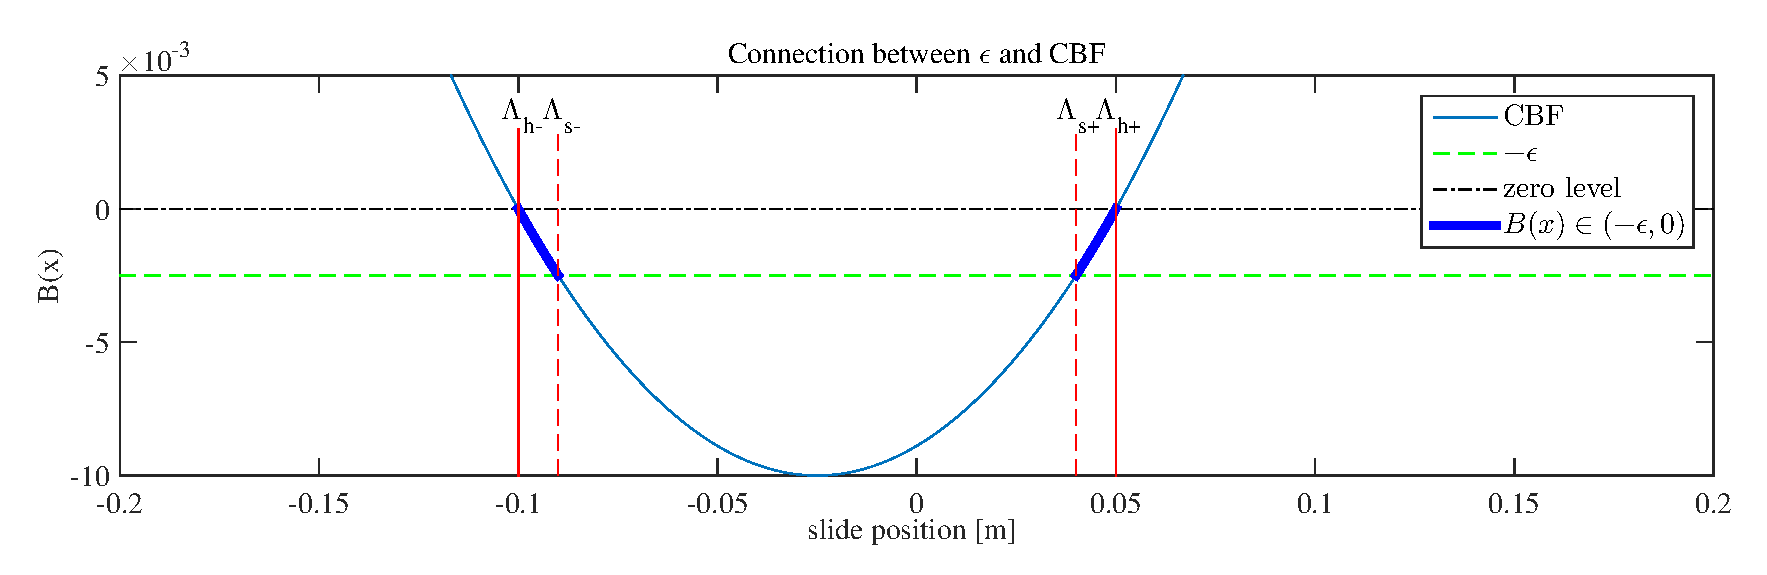
\includegraphics[scale=0.55]{epsilon_plot.eps}
	\caption{Connection between $\epsilon$ and CBF. MATLAB script and plot details can be found in \autoref{app:cd} as \texttt{matlab\_scripts/plot\_epsilon/plot\_epsilon\_slide\_1d.m}}
	\label{fig:epsilon_plot}
\end{figure}
%
%
% 
A block diagram is depicted in \autoref{fig:controlsystem}.
\begin{figure}[H]
	\center
		\includegraphics[scale=1]{control_system.pdf}
	\caption{Block diagram of the control system for slide position. MATLAB implementation is found in \autoref{app:slide_implement_1}.}
	\label{fig:controlsystem}
\end{figure}
\subsection*{Uniform Construction of $k_0$}
The control law ensuring safety can be found as \citep{bib:org_control}:
\begin{flalign}
k_0(x) = \begin{cases}
-\dfrac{L_fB(x)+ \sqrt{(L_fB(x))^2 + \kappa^2(L_gB(x))^TL_gB(x)}}{(L_gB(x))^TL_gB(x)}L_gB(x) &\text{if} \mm L_gB(x) \neq 0 \\
0  &\text{if} \mm L_gB(x) = 0
\end{cases}
\label{eq:control_law}
\end{flalign}
$\kappa$ is a design variable. High values of $\kappa$ implies increased aggressiveness. \Autoref{eq:control_law} ensures indeed safety for the closed loop system $\dot{x} = f(x)+g(x)k_0(x)$. This is easily proven as:
\begin{flalign*}
L_{f_{cl}}B(x) = L_fB(x) + L_gB(x)k_0(x)
\end{flalign*}
For $L_gB(x) \neq 0:$
\begin{flalign*}
L_{f_{cl}}B(x) &= L_fB(x) + L_gB(x) \left( -\dfrac{L_fB(x)+ \sqrt{(L_fB(x))^2 + \kappa^2(L_gB(x))^TL_gB(x)}}{(L_gB(x))^TL_gB(x)}L_gB(x) \right)  \\
&= L_fB(x) - (L_gB(x))^TL_gB(x) \dfrac{L_fB(x) - \sqrt{(L_fB(x))^2 + \kappa^2(L_gB(x))^TL_gB(x)}}{(L_gB(x))^TL_gB(x)}   \\ 
&= L_fB(x) - L_fB(x) - \sqrt{(L_fB(x))^2 + \kappa^2(L_gB(x))^TL_gB(x)} \\
&= - \sqrt{(L_fB(x))^2 + \kappa^2(L_gB(x))^TL_gB(x)} \mm \leq 0 \mm \forall \mm x
\end{flalign*}
As all terms within the square root are squared, no imaginary numbers occur, as a result $L_{f_{cl}}B(x) \leq 0$ 

According to \autoref{eq:control_law}, when $L_gB(x) = 0$:
\begin{flalign*}
L_{f_{cl}}B(x) = L_fB(x) + L_gB(x)\cdot 0 = L_fB(x)
\end{flalign*}
As $L_fB(x)$ is constructed such that $L_gB(x) = 0 \hspace{0.15cm} \Rightarrow \hspace{0.15cm} L_fB(x) < 0 $. 
\subsection{Construction of $K$ and $\bar{N}$ based on 1D Model}
The system is approximated to a linear system on the form $\dot{x}=Ax+Bu$, thus pole placement can be used. No constraints to the constant feedback matrix $K$ will be outlined except stability. It will therefore be determined from the pole placement method where a closed loop pole that is ten times faster than the open loop pole will be placed. Ackermann's formula can be used \citep{bib:acker}:
\begin{enumerate}
\item Identify the desired closed loop polynomial as $A_{cl}(s) = s^n + a_{c(n-1)}s^{n-1}  +  \cdots + a_ {c1}s + a_{c0}$: 
\begin{flalign*}
A_{cl}(s) = s + 10\,\tau^{-1}
\end{flalign*}
\item Identify the open loop polynomial as $A_{ol}(s) = s^n + a_{n-1}s^{n-1} +  \cdots + a_1s + a_0$: 
\begin{flalign*}
A_{ol}(s) = \lambda + \tau^{-1}
\end{flalign*}
\item Compute the feedback matrix in controllable canonical form:
\begin{flalign*}
 \bar{K}^T = \begin{bmatrix}   
 \bar{k_1} \\
 \vdots \\
 \bar{k_n}
 \end{bmatrix} = \begin{bmatrix}
 a_{c0} - a_0 \\
 \vdots \\
 a_{c(n-1)} - a_{n-1}
 \end{bmatrix} \kk \Rightarrow  \kk \bar{K}^T = 10\,\tau^{-1} - \tau^{-1} = 9\,\tau^{-1}
\end{flalign*}
\item Compute the similarity transform $Q$ recursively as:\\ 
\begin{minipage}[t]{0.3\textwidth}
\begin{flalign*}
&Q = \begin{bmatrix}
q_1 & q_2 & \cdots & q_n
\end{bmatrix} \\
&\text{where:}\\
&\kk q_n = B \\
&\kk q_{j-1} = A\,q_j + a_{j-1}B\\
{\color{white}{white}}\hspace{-0.5cm}
\end{flalign*}
\end{minipage}
\begin{minipage}[t]{0.1\textwidth}
\begin{flalign*}
\Rightarrow
\end{flalign*}
\end{minipage}
\begin{minipage}[t]{0.2\textwidth}
\begin{flalign*}
Q = \tau^{-1}
\end{flalign*}
\end{minipage}
\item Compute the feedback matrix as:
\begin{flalign*}
K = \bar{K}\,Q^{-1} = 9\,\tau^{-1}\dfrac{1}{\tau^{-1}} = 9
\end{flalign*}
\end{enumerate}
The constant feedback matrix, $\bar{N}$, can be computed as \citep{bib:Nbar}:
\begin{flalign*}
\bar{N} = - \left( C\,A_{cl}^{-1}\,B \right)^{-1} =  - \left( C\,(A-B\,K)^{-1}\,B \right)^{-1} = 10
\end{flalign*}
\subsection{Construction of $K$ and $\bar{N}$ based on 2D Model}
\section{MATLAB Results}
The results based on the implemented controller found in \autoref{app:slide_implement_1} is described and analysed here.
\subsection{MATLAB Results based on 1D Model}
The state trajectory composing slide position is plotted in \autoref{fig:trajectory1}
\begin{figure}[H]
	\center
		\includegraphics[scale=0.5]{trajectory_slide.eps}
	\caption{State trajectory for slide position for $\kappa=1$. MATLAB implementation can be found in \autoref{app:slide_implement_1}. The plot is based on forward euler with a sampling rate of $1\,$kHz. It is seen how the correct position is obtained in the interval $[\Lambda_{s-}:\Lambda_{s+}$]. When setpoints are given outside the safe area, the safety controller ensures that the hard boundaries $\Lambda_{h+}$ and $\Lambda_{h-}$ are not exceeded at any time and that the position founds an equilibrium at some arbitrary state.}
	\label{fig:trajectory1}
\end{figure}
Varying $\kappa$ increases the aggressivity of the safety controller and can create fluctuations in the transition area if the sampling area is too low. Likewise $\sigma(x)$ will fluctuate along with an increased $\kappa$. One must be careful when increasing $\kappa$ when the sampling rate is relatively low. %The effect of increasing $\kappa$ ten times is shown in \autoref{fig:trajectory2}.
%\begin{figure}[H]
%	\center
%		\includegraphics[scale=0.5]{trajectory_slide_kappa_10.eps}
%	\caption{State trajectory for slide position for $\kappa=10$ based on same control law and model as \autoref{fig:trajectory1}. It is seen how the safety controller is more aggressive.}
%	\label{fig:trajectory2}
%\end{figure}

To verify that \autoref{req2} is fulfilled in the simulation, the Lie derivatives are plotted in \autoref{fig:lie1}.
\begin{figure}[H]
	\center
		\includegraphics[scale=0.5]{Lie_slide_1d.eps}
	\caption{Lie derivatives of the CBF along the vector fields $f(x) = Ax$ and $g(x)=B$. It is seen that $L_gfB(x) \neq 0 \,\, \forall x \neq \frac{-b}{2a}$ which essentially fulfils \autoref{req2}.}
	\label{fig:lie1}
\end{figure}
It is from \autoref{fig:lie1} seen that $L_gB(x) \neq 0 \,\, \forall x \neq -b/(2a)$ which essentially fulfils \autoref{req2}. Indeed, even if the entire range $[\Lambda_{h-}:\Lambda_{h+}]$ belongs to $\mathcal{X}$, the chosen CBF would have been valid because the only place where $L_gB(x) = 0$ is at the critical point. Note also that the Lie derivatives are independent of the scalar $\kappa$.
For the record, the control signal is plotted in \autoref{fig:control1}.
\begin{figure}[H]
	\center
		\includegraphics[scale=0.5]{control_slide_1.eps}
	\caption{Control signal for $\kappa=1$. It is seen how the controller counteracts the large difference in setpoints given and in that way ensures safety. It is seen that when the absolute value of the setpoints are increased then $u(x)$ increases accordingly. The plot is ideal as no saturation constraints are given.}
	\label{fig:control1}
\end{figure}
It is seen from \autoref{fig:control1} how the control signal reacts instantaneously and quite aggressive when $\Lambda_s$ is exceeded to counteract the large difference in setpoints given. It is also noted how the controller eventually settles smootly even when setpoints are given in the interval $[-\infty:\Lambda_{s-}]$ and $[\Lambda_{s+}:\infty]$. However, as the setpoints approaches $\pm \infty$, the sampling rate must also converge towards infinity. This is obviously not a realistic scenario as the slide movement is physically constrained.
\subsection{MATLAB Results based on 1D Model}

\section{Implementation on the Da Vinci Robot}
\subsection{Implementation on the Da Vinci Robot based on 1D Model}

\subsection{Implementation on the Da Vinci Robot based on 2D Model}
